%%%%%%%%%%%%%%%%%%
\subsection[Exploration]{Exploration$^{\star,\circ}$}\label{alg:exploration} % this indicates that it is written by @adaudrich and small adjustments have been done by @0nse.
One precondition of the Agents on Mars Scenario is that all agents start with an empty belief base.
No agent knows about its local or global environment.
Every agent gets beliefs about its local environment quickly by receiving percepts from the server.
But the agent stays unaware of the global environment.
For our strategies it is crucial to have as much information of the overall environment as possible.
This is necessary to e.g.\ find the shortest path from one vertex to another or to calculate a zone returning high scores.
To achieve this, it is mandatory to somehow store information about the map like its vertices, edges between vertices, paths and agent positions.

The following subsections describe our different approaches on how to store and process this information.
In more detail, the first section, \autoref{alg:map_cartographer}, presents our first approach with its up- and down-sides.
After that a basic overview of our initial map building approach is given in \autoref{alg:map_dv}.
Finally, this section concludes with a description of the second approach we used and finally stuck to in \autoref{alg:map_javamap}.

%%%%%%%%%%%%%%%%%%
\subsubsection[Cartographer Agent]{Cartographer Agent$^{\star,\circ}$}\label{alg:map_cartographer}
Very early in our development process we decided that we wanted to store all information about the map in a central place.
This means we were not interested in each agent storing all map data in its own belief base.
The intention behind this decision was to reduce the effort in synchronising and maintaining data between the single agents.
This section presents our initial approach which was to install one additional, omniscient agent which we called the \emph{cartographer agent}.
It was a separate agent existing in the background and was independent from our 28 agents of the simulation.
The cartographer agent stored map information and had the task to calculate shortest paths between given vertices.
Said map information included vertex values, edges between them and their associated traversing costs.
Every agent told the cartographer agent about its environment related beliefs and the cartographer agent stored these beliefs.
Environment related beliefs are given in the listing below:
\begin{lstlisting} [caption={Map exploration related beliefs}, label={lst:dv_exploration_beliefs}]
   visibleEntity(<Vehicle>, <Vertex>, <Team>, <Disabled>).
   position(<Vertex>).
   visibleVertex(<Vertex>, <Team>).
   probedVertex(<Vertex>, <Value>).
   visibleEdge(<VertexA>, <VertexB>).
   surveyedEdge(<VertexA>, <VertexB>, <EdgeCosts>).
\end{lstlisting}

If an agent needed to know a shortest path, it queried the cartographer agent and got the shortest path as an answer.
The agent could also query the cartographer agent for getting to know whether a vertex was already probed or surveyed.
See \autoref{fig:map:com1} for the communication process of our first approach.
\autoref{fig:map:comp1} shows the distribution of the single components related to map exploration.
\begin{figure}
  \centering
  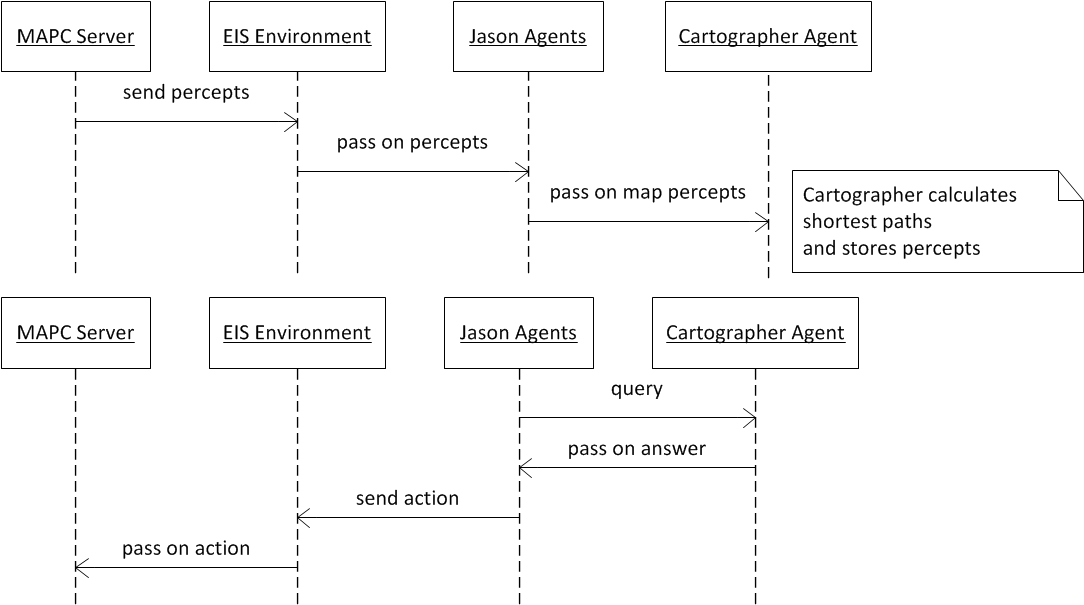
\includegraphics[width=\linewidth]{images/map_com_1.png}
  \caption{Initial communication approach for map generation.}
  \label{fig:map:com1}
\end{figure}

\begin{figure}
  \centering
  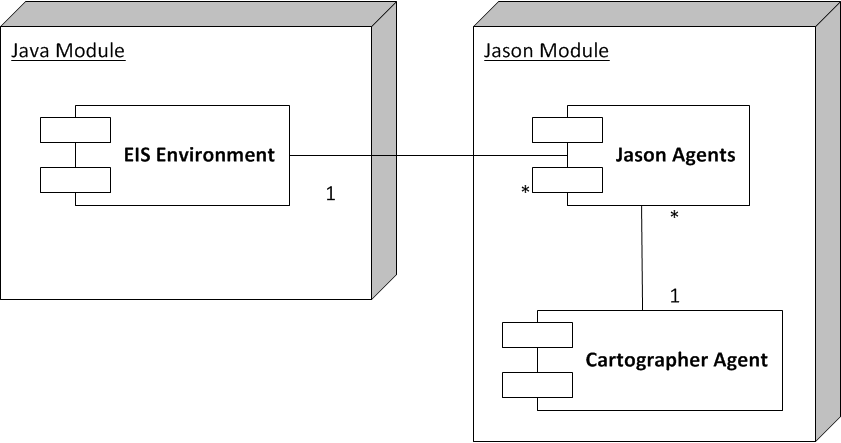
\includegraphics[width=0.7\linewidth]{images/map_comp_1.png}
  \caption{Distribution of components between Jason and Java in our first approach.}
  \label{fig:map:comp1}
\end{figure}

Shortly after implementing this approach, we encountered two major problems, which both resulted in serious performance issues.
One problem came from our implementation of the pathfinding to determine the shortest path between two vertices.
Although we used the Dijkstra's algorithm, which is an efficient algorithm for this task, we encountered performance issues.
The reason was that the pathfinding algorithm was executed every time an agent asked for a shortest path.
This led to a lot of redundant calculations and processing in the cartographer agent.

The second problem was related to communication between agents.
To understand the latter problem, one needs to know that Jason uses a mail box system for communication between agents.
This means that every message by an agent is queued in the receiver's message inbox.
In every Jason lifecycle only one message is processed.
Although a Jason lifecycle is a lot shorter than a server step, after some execution time the cartographer agent processed fewer messages than it received.
Both issues resulted in blocked agents, which had been waiting for the response to their queries for several steps.

The following example should illustrate this problem.
An exploring agent comes to an unvisited vertex.
The first thing it does, is to ask the cartographer agent, whether this vertex was surveyed in the meantime.
After it gets the answer it surveys the vertex or asks the cartographer agent for the next not surveyed vertex and travels there.
Then the whole procedure starts again.
As one can see, at least two messages are needed each time and hence there are two possible bottlenecks.
The first one is the query for the state of a vertex and the second is the query for the next not surveyed vertex, which includes calculating the shortest path to this vertex.
If the agent surveyed the vertex, it will additionally have to inform the cartographer agent about the new information.
This information is received and will be forwarded by the respective agent when the next step begins.
Due to the Jason communication approach this results in the cartographer not being able to handle queries immediately.
In our tests we saw answer times for queries around ten till twenty server steps.
This lead to our agents being idle most of the time, waiting for answers from the cartographer agent.
Obviously, this would be suboptimal for the competition.
The next section describes our second approach which tries to reduce the calculation overhead for the cartographer agent when calculating shortest paths.

%%%%%%%%%%%%%%%%%%
\subsubsection[Distance-Vector Routing Protocol]{Distance-Vector Routing-Protocol$^{\star,\circ}$}\label{alg:map_dv}
This section presents our next approach which tried to solve the problem with repeating calculations of shortest paths.
It was first built to work together with the cartographer agent but was later used independently.
We decided to calculate all shortest paths as early as possible and store these paths together with other information in a network of what we called \emph{node agents}.
A node agent is an agent representing one vertex of the scenario map and storing information about this vertex.
All percepts perceived by our 28 agents were passed on to the node agents.
To make it easier to address node agents, we named node agents like the vertex they represented.
Node agents stored all their neighbours in a neighbour-list belief \texttt{neighbours([<ListOfNeighbours>])}.
Additionally, they stored all available paths to other vertices as shortest path beliefs \texttt{minStepsPath(<Destination>, <NextHop>, <Hops>, <CostToNextHop>)}.
Similarly, they stored all available paths to other vertices as cheapest path beliefs \texttt{minCostPath(<Destination>, <NextHop>, <TotalCosts>, <CostToNextHop>)}.
The addition of a cheapest path belief would allow an agent to travel towards a destination vertex while having to use the fewest energy.
Hence, the agent would be able to travel to a vertex with recharging more seldom at the expense of possibly needing more hops to reach it.
In regard to exploration and zoning, we decided that a node agent also had to store the probed value of the vertex, and whether it had already been probed or surveyed.

At first, we changed the cartographer agent's tasks, so that it only had to create the node agents at runtime and redirect queries.
Hence, the cartographer agent became an intermediate agent ensuring that the node agents existed.
All map related percepts were now redirected by the cartographer agent to the respective node agents.
Agents would query node agents directly, when they were looking for how to reach a specific vertex.
This only happened, when agents could not see a not surveyed vertex to explore next.
Yet, they had to ask the cartographer agent for a list of not surveyed vertices in a farther distance.
That way, we were able to ensure the existence of a node agent prior to a regular agent communicating with this node agent.
\autoref{fig:map:com2} shows the second approach we used and \autoref{fig:map:comp2} the corresponding distribution model.
\begin{figure}
  \centering
  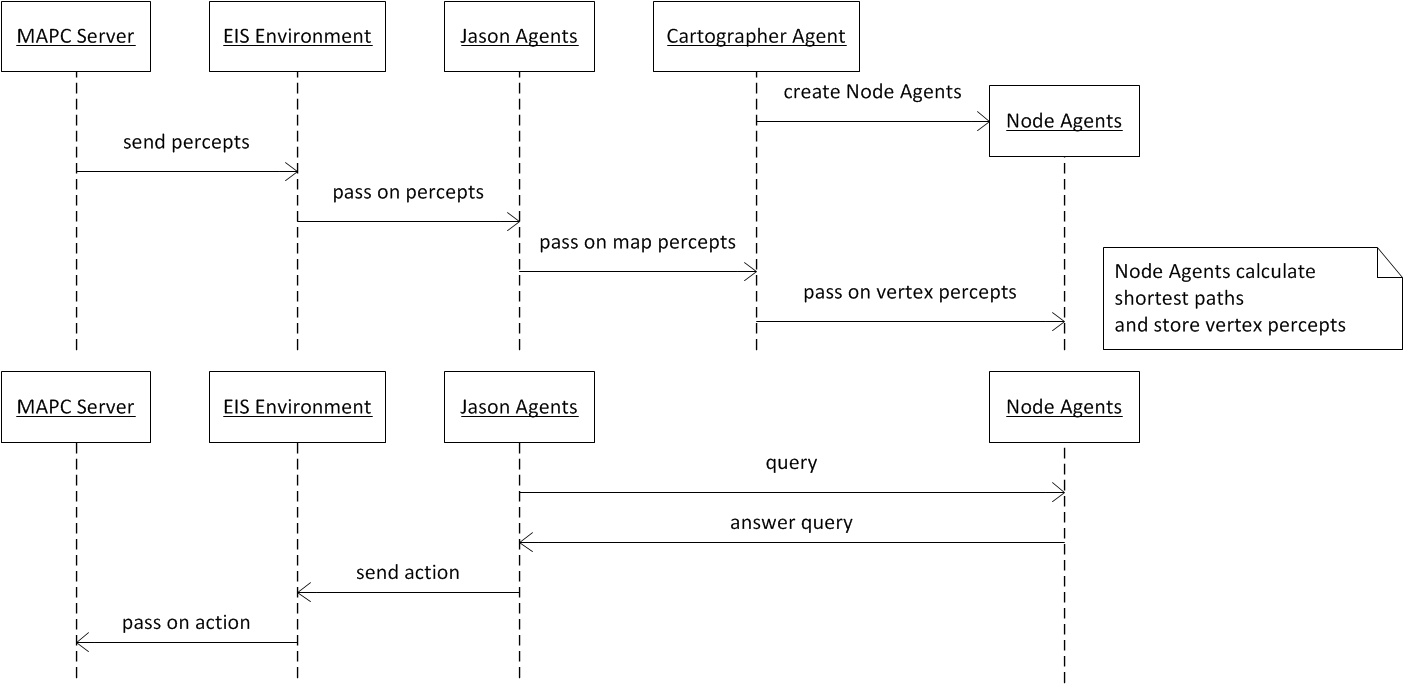
\includegraphics[width=\linewidth]{images/map_com_2.png}
  \caption{Second communication approach for map generation with using the cartographer agent.}
  \label{fig:map:com2}
\end{figure}

\begin{figure}
  \centering
  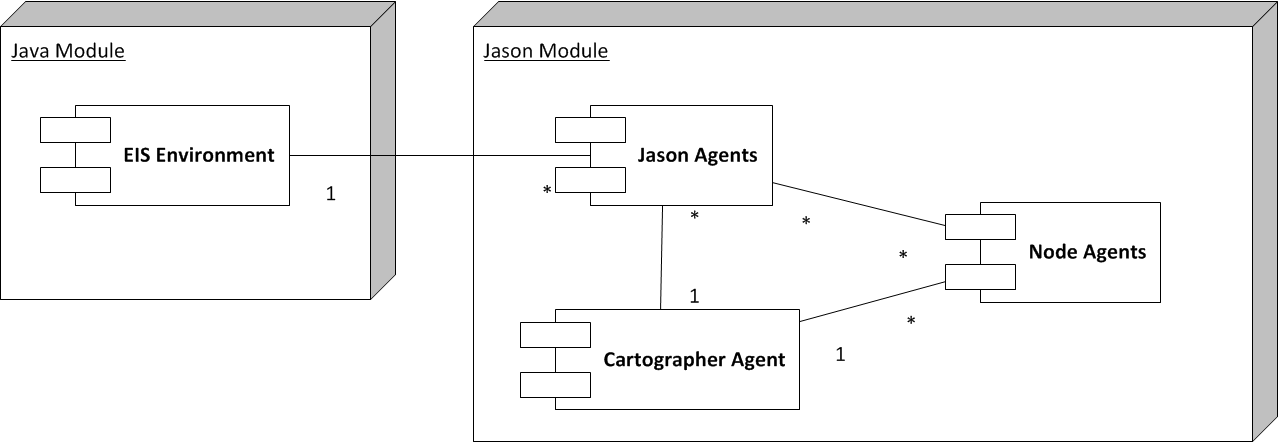
\includegraphics[width=\linewidth]{images/map_comp_2.png}
  \caption{Distribution of map components in our second approach with using the cartographer agent.}
  \label{fig:map:comp2}
\end{figure}

The dynamic creation of node agents during runtime was done because the number of vertices is not known until the simulation start.
As the creation of a few hundred agents takes some time itself, it was not possible to create the node agents during runtime after the simulation started.
But having the cartographer agent function as an intermediary made it another bottleneck.
So, we later eliminated this agent completely and simply created $625$ node agents before the simulation started.
This is the maximum number of possible vertices.
For the sake of performance, we here accepted to have some idling node agents which would not participate with any other agent.
We also experimented with removing unnecessary node agents once we knew how many vertices the simulation had.
But this had no noticeable impact on the performance or stability of the system for what reason we removed it shortly after again.

\begin{samepage}
The following list shows an example belief base of a node agent \texttt{v1}:
\begin{itemize}
  \item \texttt{neighbours([v2, v3]).}
  \item \texttt{probed(true).}
  \item \texttt{probedValue(7).}
  \item \texttt{surveyed(true).}
  \item \texttt{minStepsPath(v1, v1, 0, 0).}
  \item \texttt{minStepsPath(v2, v2, 1, 3).}
  \item \texttt{minStepsPath(v10, v2, 4, 3).}
  \item \texttt{minStepsPath(v8, v3, 3, 2).}
\end{itemize}
\end{samepage}
A query for a shortest path to \texttt{v8} would then look like this:
\begin{lstlisting}[caption={Query for shortest path from \texttt{v1} to \texttt{v8}}, label={lst:dv_shortestPath_query}]
  .send(v1, askOne, minStepsPath(v8, NextHop, _, CostToNextHop)).
\end{lstlisting}
After looking up the belief in its belief base the node agent would unify the parameter \texttt{NextHop} with \texttt{v3} and \texttt{CostToNextHop} with \texttt{2} and respond this to the querying agent.

For propagating data between these node agents we used a modified \emph{Distance-Vector Routing Protocol} \cite{dvrp} (short: DV)
DV is a routing protocol based on the Bellman-Ford algorithm and normally has its use in packet-switched networks.
It can be executed on a network of nodes.
The basic idea is that each node informs all of its neighbour nodes about its belief base.
The informed nodes then update their belief base and also inform all of its neighbours and so on.
Because this algorithm has no loop detection for larger networks, we had to implement some kind of break condition for the algorithm.
We used the value of the calculated shortest path or the calculated cheapest path respectively as a termination condition.
If a new calculated path to another node agent was shorter than the already known path, then the node agent informed its neighbours.
Otherwise it would do nothing.
At some point all information and paths are propagated through the whole network and all nodes have a consistent belief base.
\autoref{fig:dv} illustrates the algorithm for a small set of four neighbour nodes.

\begin{figure}
  \centering
  \caption{Executing the Distance-Vector Routing Protocol algorithm as described in \autoref{alg:map_dv} on a small network of four nodes to calculate the shortest paths.
           Each node has a table attached, containing all accessible nodes.
           The first parameter is the destination node, the second one is the node to pass through and the third parameter shows the overall distance to the destination.
           For more compact display, we left out the parameter showing the cost of the edge to the next hop.\label{fig:dv}}
    \begin{subfigure}{.45\textwidth}
        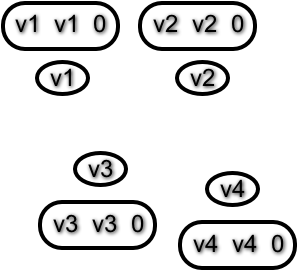
\includegraphics[width=\textwidth] {images/dv0.png}
        \caption{Initial set of node agents with their belief base.
                 Each node agent knows only about itself and the shortest path to itself.
                 The travelling costs to itself are zero.}
    \end{subfigure}\quad
    \begin{subfigure}{.45\textwidth}
        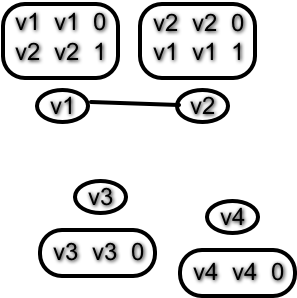
\includegraphics[width=\textwidth] {images/dv1.png}
        \caption{The node agents \texttt{v1} and \texttt{v2} are informed that they are neighbours.
                 So they know that there must be a path to the other node agent.
                 Because they are direct neighbours they are one hop away.
                 As \texttt{v3} and \texttt{v4} are not connected to the network at this point, so they will not be informed about the path between \texttt{v1} and \texttt{v2}.}
    \end{subfigure}

    \begin{subfigure}{.45\textwidth}
       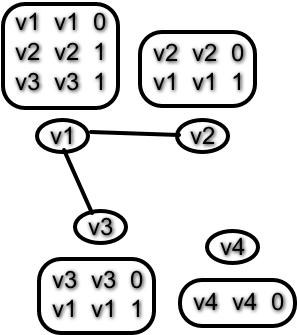
\includegraphics[width=\textwidth] {images/dv2.png}
       \caption{Now \texttt{v3} is added to the network by informing \texttt{v3} and \texttt{v1} about their neighbourhood relation.
                At first only \texttt{v1}  and \texttt{v3} update their belief base.}
    \end{subfigure}\quad
    \begin{subfigure}{.45\textwidth}
        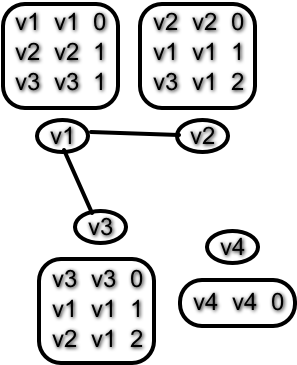
\includegraphics[width=\textwidth] {images/dv3.png}
        \caption{In the next step \texttt{v2} is informed about the path from \texttt{v1} to \texttt{v3}.
                 The shortest path to \texttt{v3} from \texttt{v2} is now known to be 2 hops away, going over \texttt{v1}.}
    \end{subfigure}
\end{figure}
\clearpage
\begin{figure}
  \centering
    \ContinuedFloat % continue from previous page
    \begin{subfigure}{.45\textwidth}
        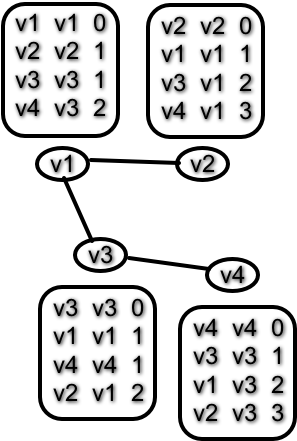
\includegraphics[width=\textwidth] {images/dv4.png}
        \caption{Adding the knowledge about an edge between \texttt{v3} and \texttt{v4} will make all node agents update their belief base.}
    \end{subfigure}\quad
    \begin{subfigure}{.45\textwidth}
        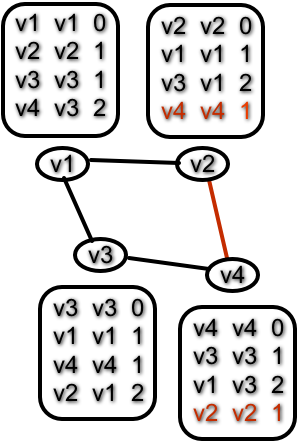
\includegraphics[width=\textwidth] {images/dv5.png}
        \caption{In the last step, \texttt{v2} and \texttt{v4} are informed of being neighbours.
                 Because of that, the shortest path between both node agents changes and is updated.
                 The paths for the other node agents stay unchanged, because they cannot improve.}
    \end{subfigure}
    \phantomcaption
\end{figure}

By distributing the information from the cartographer agent onto a huge network of node agents, we also distributed the load from one agent between the respective node agents.
But we still had queries which were not answered immediately, because now we had a lot of communication going on between node agents.
Around 400 Jason agents were calculating shortest and cheapest paths in parallel within the node agent networks.
At the same time, they received new information by the exploring agents.
Although this information was redundant in most cases, it still had to be processed.
This led to a high load on our system.
To reduce the load, we decided to prefer the shortest over the cheapest paths and henceforth only calculate the shortest paths.
We made this decision because we found losing a step due to travelling a path with more hops was worse than having to recharge more often.
The reason for this is that recharging returns half of the maximum energy to the agent with which it can pass multiple hops most of the time.

Next, we reduced communication between node agents and real agents.
At all times, the necessary map information was first received from the Java EIS Environment module.
The Java EIS Environment module is our interface to communicate with the MAPC server.
Through this interface we got agent percepts from the server and transmitted actions to the server.
Originally, the map information was blindly transmitted to the agents who perceived this information.
They then themselves passed the information on to the node agents.
Our change here was to add a filter to this module which would only transmit new information and would send it directly to the respective note agents.
Since the message boxes were no longer flooded, communication between agents got a lot better.

But two reasons made us discard this approach as well and change to a solution based entirely on Java.
First, we were not able to reduce the load on our system sufficiently by these changes.
Further, we observed that some beliefs were not received by the node agents.
Even worse, over time beliefs disappeared from node agents belief bases.
Due to the constant high workload on our system, we saw that agents sent actions to the server too late, which led again to a lot of idle steps of our agents.
The next section presents the solution which we used for the competition.

%%%%%%%%%%%%%%%%%%
\subsubsection[JavaMap]{JavaMap$^{\star,\circ}$}\label{alg:map_javamap}
We decided to implement the whole map module in Java.
This solved all of the previously described problems.
The JavaMap module gets its map information directly from the Java EIS Environment module.
It is queried through internal actions by the Jason agents which were presented in \autoref{fun:apl_jason}.
Internally the JavaMap creates and manages a list of vertex-objects which are similar to the node agents from our previous approach.
Every vertex stores a list of all paths it knows and all vertex information.
This includes the one-hop neighbourhood and the probed value of the vertex.
During our tests we often encountered the problem that multiple agents where sent to the same node.
To solve this, we extended the functionality of our JavaMap with a mechanism to prevent agents from traveling to the same node when exploring, probing, repairing or attacking. To do this we used internally a reservation list for each task. In this list we kept the information which agent was doing which task, e.g.\ we saved in the survey list that an agent reserves surveying a node. If another agent asks for a not already surveyed vertex, the nearest not surveyed vertex will be first checked with the reservation list. If the vertex is not in the list it will be assigned to the agent and saved to the list, otherwise the next nearest not surveyed vertex will be checked, and so on. This list is reset at the beginning of each step, so that agents can react on environment changes, like already surveyed vertices or enemies in their path to the vertex, in every step.

\autoref{fig:map:com3} shows how the map percepts are now passed to the JavaMap and how Jason agents query the JavaMap.
\begin{figure}
  \centering
  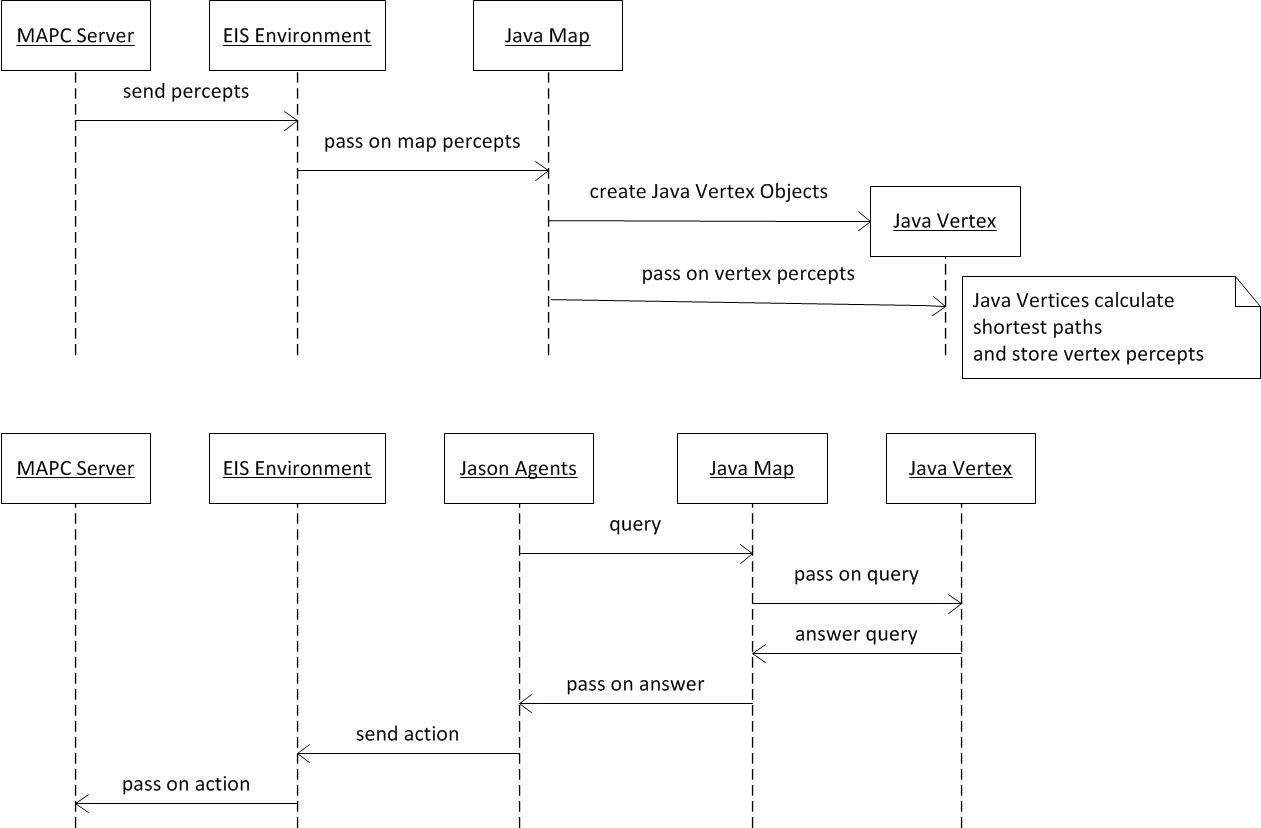
\includegraphics[width=\linewidth]{images/map_com_3.png}
  \caption{Final communication approach for map generation.}
  \label{fig:map:com3}
\end{figure}

In \autoref{fig:map:comp3} it is demonstrated how we changed the distribution of our components for map generation between Java and Jason.
Unlike the first and second approach we now have a separation of concerns.
The whole map generation and calculation is done entirely in Java and agent related actions, planning and communication entirely in Jason.
\begin{figure}
  \centering
  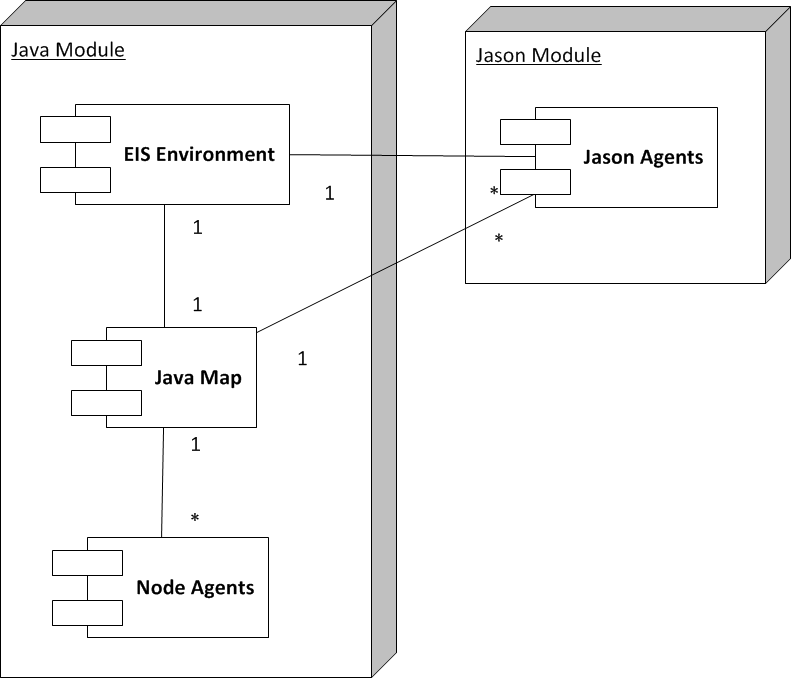
\includegraphics[width=0.6\linewidth]{images/map_comp_3.png}
  \caption{Distribution of map components in our final solution.}
  \label{fig:map:comp3}
\end{figure}

With JavaMap we found an exploration approach which is fast, stable and has a high coverage of the actual map.
Furthermore, we could be sure that all information is accessible by every Jason agent in reasonable time.
We were also able to reduce the time to receive answers to rather complex queries like paths between distant vertices.
